\chapter{CoCoME}
\label{ch:CoCoME}
The \textit{Common Component Modelling Example (CoCoME)} is a common case study on software architecture modelling \cite{CoCoMEOld}\cite{CoCoMETechnical}. In this thesis, it is used to demonstrate and validate the presented approach. Sec.\ref{sec:CoCoME:Introduction} provides a short introduction of the demonstrator, followed by a presentation of its system specifications.


\section{Introduction to CoCoME}
\label{sec:CoCoME:Introduction}
CoCoME represents a trading system as it can be found in a supermarket chain. The main task is handling and processing sales at a single store of the chain. Therefore, customers can pick goods and place them on the \textit{Cash Desk} whose main component is a \textit{Cash Desk PC}. Several other components like \textit{Bar Code Scanner}, \textit{Light Display}, \textit{Printer}, \textit{Card Reader} and \textit{Cash Box} are wired by the  \textit{Cash Desk PC}. \\
Multiple  \textit{Cash Desks} of a single store form a  \textit{Cash Desk Line}, which is connected to the  \textit{store server}. A set of stores in the CoCoME chain is organized as an enterprise where each store is connected to a single enterprise server. \\
More detailed description of the CoCoME system can be found in \cite{CoCoMEOld}\cite{CoCoMETechnical}. The next section provides information about the system requirements specifications in form of use cases.
 


\section{System specifications}
\label{sec:CoCoME:systemSpecifications}
The system specification is informal and given in the form of detailed use cases. Fig.\ref{fig:useCases} provides an overview of the use case of CoCoME. A full detailed description can be found in \cite{CoCoMEOld}.




\begin{figure}[h!]
	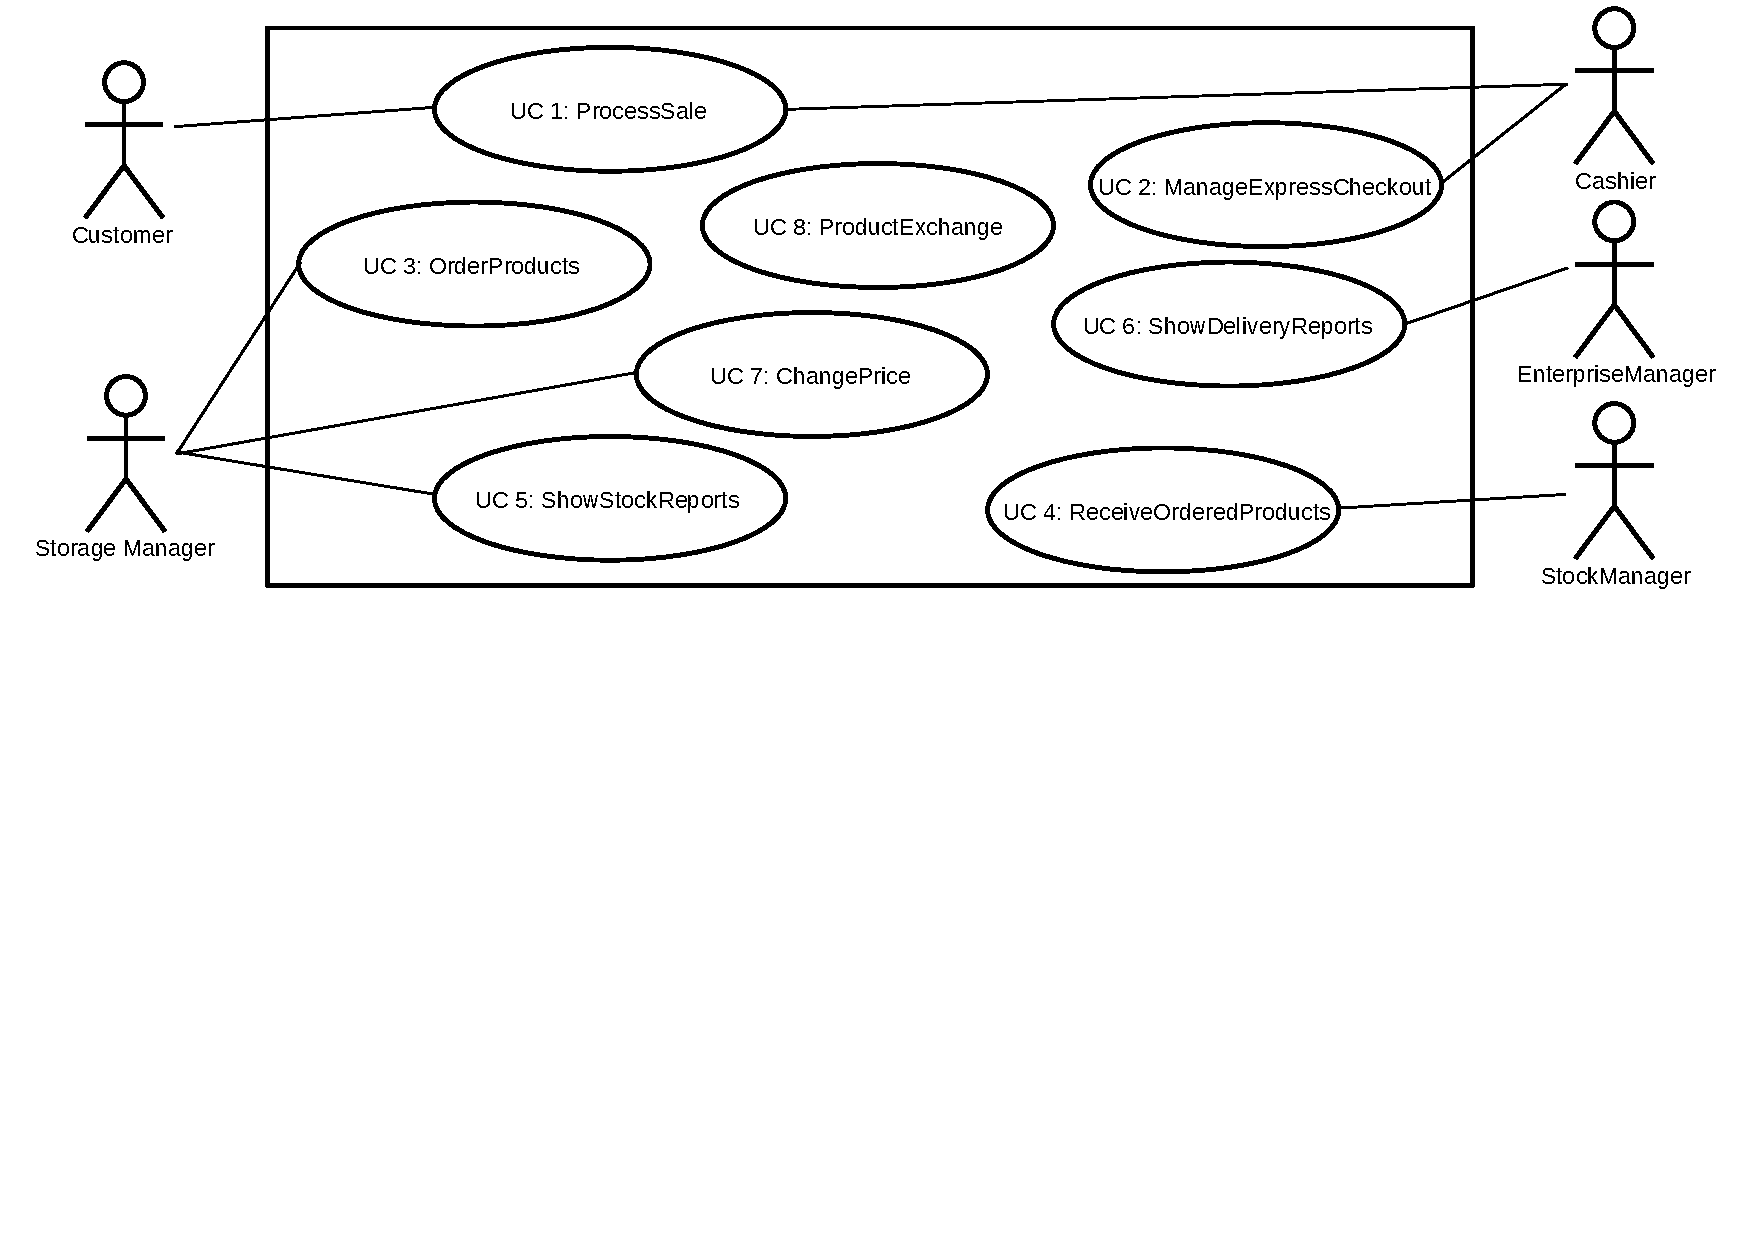
\includegraphics[width=\textwidth, trim={0 11cm 0 0}]{img/useCase.pdf}
	\caption{Use Case Diagram}
	\label{fig:useCases}
\end{figure}


\begin{description}


 \item[Use case description]~\par
\begin{itemize}
	\item \textit{Process Sale:} Handles the products a customer wants to purchase and the payment (either cash or card).

    \item \textit{Manage Express Checkout:} The cash desk switches automatically in the express mode (under certain conditions). The cashier is able to switch back in normal mode.
    \item \textit{Order Products:} A store manager can order products from suppliers.
    \item \textit{Receiver Ordered Products:} Ordered products which arrive at the store need to be checked for correctness and inventoried by the stock manager.
    \item \textit{Show Stock Reports:} A store manager can request a stock-related report for his/her store.
    \item \textit{Show Delivery Reports:} Calculation of the mean time for a delivery.
    \item \textit{Change Price:} The sale price of a product is changed.
    \item \textit{Product Exchange:} Automatic stock exchange if a store is running out of stock and other stores still have the required product
\end{itemize}


\end{description}